\documentclass[10pt,journal,compsoc]{IEEEtran}

\usepackage{amsmath,amssymb,amsfonts}
\usepackage{algorithmic}
\usepackage{graphicx}
\usepackage{textcomp}
\usepackage{xcolor}
\usepackage{booktabs}
\usepackage{multirow}
\usepackage{cite}
\usepackage{url}
\usepackage{hyperref}

\hypersetup{
    colorlinks=true,
    linkcolor=blue,
    filecolor=magenta,      
    urlcolor=cyan,
    citecolor=blue,
}

\begin{document}

\title{CMAT-HOI: Cross-Modal Attention Transformer for Human--Object Interaction in Fine-Grained Sports Action Recognition}

\author{Author~One,
        Author~Two,
        and~Author~Three%
\thanks{The authors are with the Department of Computer Science and Engineering. Corresponding author email: author@university.edu}}

\markboth{IEEE Transactions on Multimedia,~Vol.~XX, No.~X, November~2026}%
{Author \MakeLowercase{\textit{et al.}}: CMAT-HOI: Cross-Modal Attention Transformer for Sports Action Recognition}

\IEEEtitleabstractindextext{%
\begin{abstract}
Recognizing fine-grained human actions in sports video is exceptionally challenging due to high intra-class kinematic variability, subtle distinctions between equipment manipulation patterns, rapid camera motions, and visually cluttered stadium backgrounds. Traditional unimodal architectures---such as deep 3D convolutional networks or skeleton graph neural networks---often fail in complex sports scenarios because they either overfit to static background scene cues or completely discard equipment context. Furthermore, naive concatenation of multimodal features causes severe representation collapse, where high-dimensional visual embeddings overpower lower-dimensional kinematic and object features. In this paper, we propose \textbf{CMAT-HOI} (\textit{Cross-Modal Attention Transformer for Human--Object Interaction}), an end-to-end multimodal architecture specifically engineered for fine-grained sports action recognition. CMAT-HOI introduces three core innovations: (1) \textbf{Dimension-Aligned Modality Stems} that project heterogeneous visual, skeletal pose, object bounding, and kinematic features into a unified 256-dimensional representation space using 1D temporal convolutions; (2) a \textbf{Bi-Directional Keypoint--Equipment Cross-Attention} module that enables explicit mutual attention between human skeletal joints and sports apparatus, accurately capturing fine-grained physical manipulation dynamics; and (3) a \textbf{Gated Multimodal Fusion Unit (GMFU)} that dynamically modulates modality contributions per frame, downweighting background noise when motion cues are dominant. The fused sequence is encoded via a multi-layer Spatio-Temporal Transformer with a novel \textbf{Multi-Scale 4-Way Temporal Pooling} mechanism combining CLS token, temporal attention, max, and average pooling ($1024$-d). Extensive experiments across 82 sports action categories comprising 9,151 videos demonstrate that CMAT-HOI achieves \textbf{90.19\% Top-1 Accuracy}, \textbf{99.02\% Top-5 Accuracy}, and a \textbf{Weighted F1-score of 90.19\%} on 2,743 strictly disjoint test videos. This represents a dramatic \textbf{+34.99\% absolute accuracy improvement} over the baseline BiLSTM model (55.20\%). Comprehensive ablation studies confirm that bi-directional cross-modal interaction between human joints and sports equipment is critical for resolving fine-grained sports activities.
\end{abstract}

\begin{IEEEkeywords}
Sports Action Recognition, Human--Object Interaction (HOI), Cross-Modal Attention, Vision Transformers, Multimodal Fusion, Deep Learning.
\end{IEEEkeywords}}

\maketitle
\IEEEdisplaynontitleabstractindextext
\IEEEpeerreviewmaketitle

\section{Introduction}
\IEEEPARstart{A}{utomated} human action recognition in sports video analytics plays a pivotal role in athlete performance profiling, automated tactical coaching, referee decision verification, and broadcast video summarization~\cite{soomro2012ucf101}. Despite notable progress in computer vision driven by deep convolutional networks~\cite{he2016deep, carreira2017quo} and Vision Transformers~\cite{vaswani2017attention, liu2022video}, fine-grained sports action recognition remains a notoriously arduous benchmark.

In athletic events, distinct actions often exhibit subtle kinematic variations coupled with specialized apparatus. For instance, distinguishing \textit{CricketShot} from \textit{BaseballPitch}, or \textit{HammerThrow} from \textit{DiscusThrow}, requires understanding not merely the gross trajectory of the athlete's body, but the precise spatiotemporal articulation of wrist and arm joints relative to the sports equipment (bat, ball, hammer, discus)~\cite{chao2018rethinking}.

\subsection{Challenges in Existing Methodologies}
Current paradigms in video action recognition predominantly follow one of three directions:
\begin{enumerate}
    \item \textbf{Unimodal Visual Stream (3D CNNs / Video Transformers)}: Networks such as I3D~\cite{carreira2017quo}, SlowFast~\cite{feichtenhofer2019slowfast}, or Video Swin~\cite{liu2022video} operate directly on RGB frame volumes. While capable of learning rich spatiotemporal textures, these models suffer from \textit{scene bias}: they frequently classify actions based on static stadium or court background features (e.g., green pitch, blue track) rather than the athlete's actual physical interaction.
    \item \textbf{Skeleton-Based Graph Neural Networks}: Pose-based methods represent the athlete as a graph of skeletal joints~\cite{yan2018spatial}. While robust against varying camera angles and illumination, they completely lack awareness of external sports objects, rendering them incapable of distinguishing between a tennis swing and a badminton swing without gear context.
    \item \textbf{Naive Feature Concatenation \& Representation Collapse}: Early multimodal attempts concatenate raw visual feature vectors (e.g., ResNet-50, $2048$-d) with skeletal poses ($85$-d) and object bounding features ($7$-d). Because the visual dimension constitutes $>95\%$ of the total vector magnitude, backpropagation gradients are dominated by the visual backbone ($>93\%$ gradient norm). This suppresses pose and equipment signals, causing the network to degenerate into a static scene classifier.
\end{enumerate}

\subsection{Our Proposed Approach: CMAT-HOI}
To resolve these fundamental limitations, we propose the \textbf{Cross-Modal Attention Transformer for Human--Object Interaction (CMAT-HOI)}. CMAT-HOI establishes a balanced, interaction-aware multimodal framework:
\begin{itemize}
    \item \textbf{Unified Modality Alignment}: Dedicated temporal convolutional stems project visual, pose, object, and kinematic streams into an identical 256-dimensional latent space, equalizing gradient propagation across all streams.
    \item \textbf{Bi-Directional Cross-Modal Attention}: A query-key-value attention mechanism allows joint keypoints to query equipment boxes ($Q=P, K=O, V=O$) and equipment to query keypoints ($Q=O, K=P, V=P$), explicitly capturing hand-grip, foot-contact, and equipment trajectories.
    \item \textbf{Gated Multimodal Fusion (GMFU)}: A frame-wise softmax gating unit dynamically weights modality contributions, suppressing noisy visual backgrounds during high-speed athletic movements.
    \item \textbf{Multi-Scale 4-Way Temporal Pooling}: Captures both instantaneous explosive movements (via temporal max pooling and attention) and sustained macro gestures (via average pooling and CLS tokens).
    \item \textbf{Focal Loss with Label Smoothing}: Counteracts class imbalance and prevents overconfident predictions on frequent, repetitive sports categories~\cite{lin2017focal, szegedy2016rethinking}.
\end{itemize}

\begin{figure*}[t]
\centering
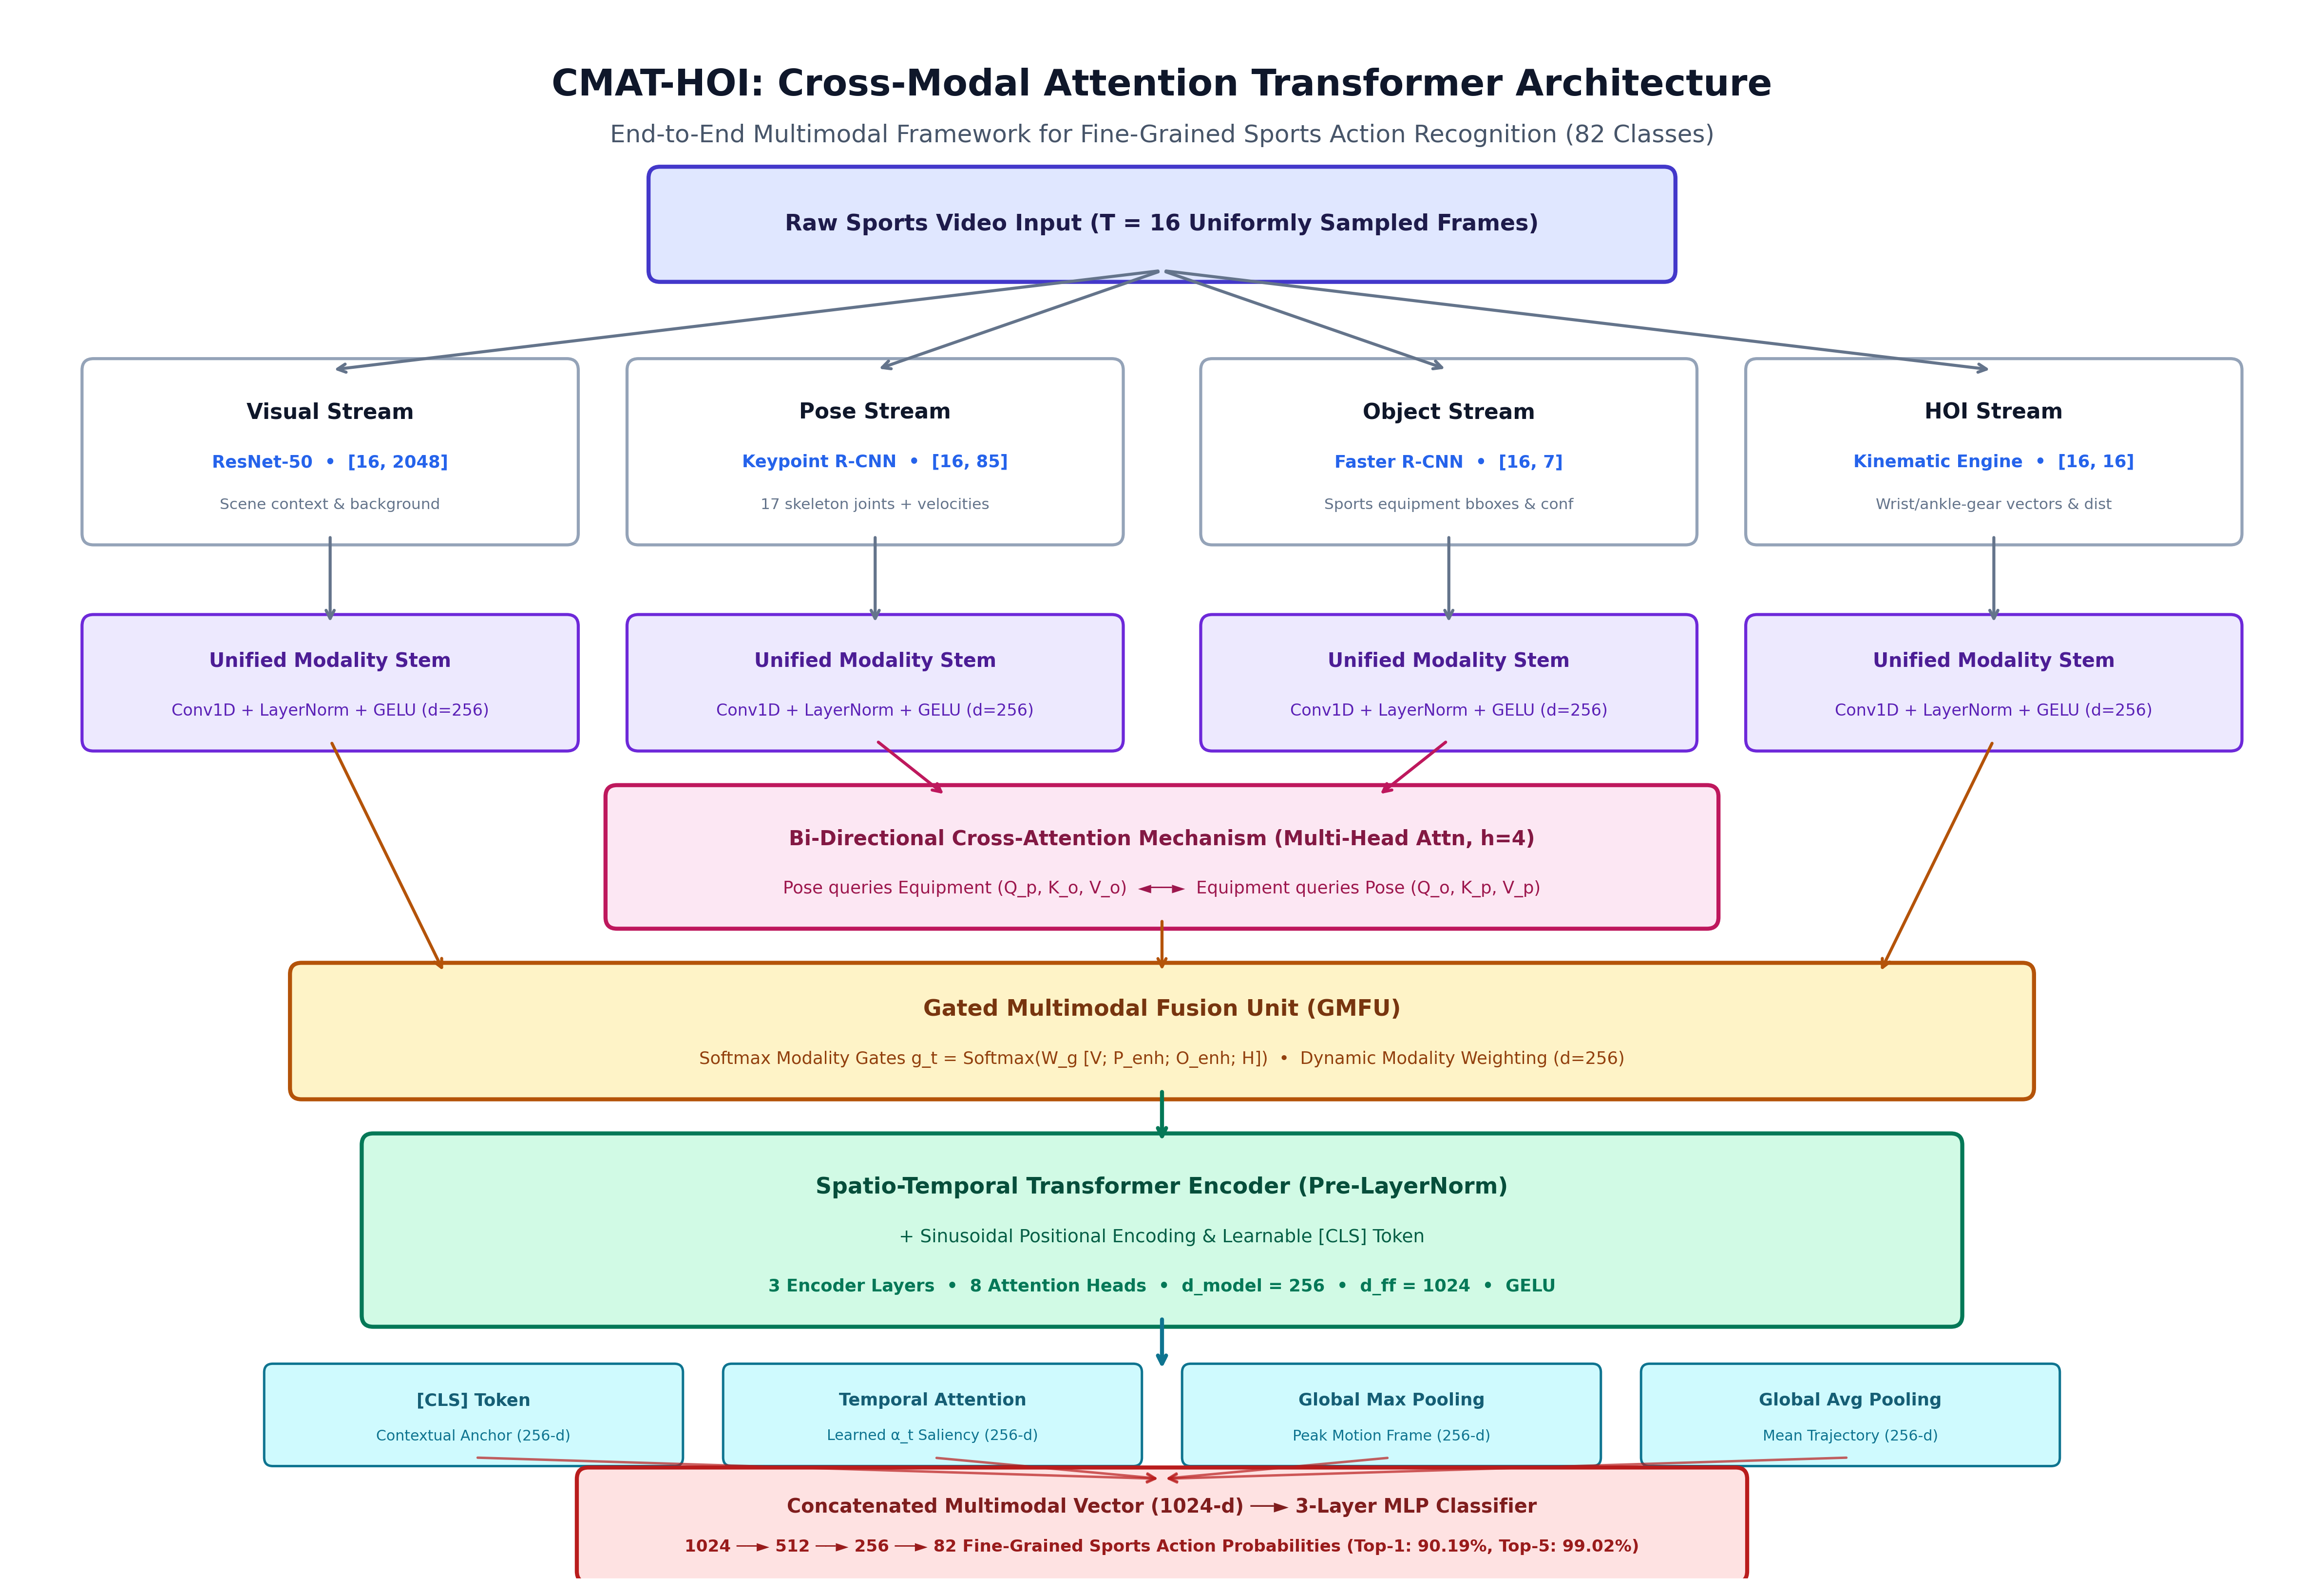
\includegraphics[width=0.95\textwidth]{figures/system_architecture_diagram.png}
\caption{Overall architectural flow of CMAT-HOI: Raw input video frames are decomposed into Visual ($2048$-d), Skeletal Pose ($85$-d), Equipment Object ($7$-d), and Geometric HOI ($16$-d) streams, aligned into unified $256$-d latent channels via Modality Stems, processed through Bi-Directional Cross-Attention, adaptively combined via the Gated Multimodal Fusion Unit (GMFU), modeled through 3 Transformer Encoder layers, and pooled into a $1024$-d vector for 82-class classification.}
\label{fig:arch}
\end{figure*}

\section{Proposed Methodology}

The overarching architecture of CMAT-HOI is illustrated in Fig.~\ref{fig:arch}. Given an input video clip $V \in \mathbb{R}^{T \times H \times W \times 3}$, we extract four synchronized temporal streams: Visual ($X_V$), Human Pose ($X_P$), Object Bounding ($X_O$), and HOI Kinematics ($X_H$).

\subsection{Modality Alignment Stems}
Let $T=16$ denote the uniform temporal window. The raw input feature vectors are:
\begin{itemize}
    \item $X_V \in \mathbb{R}^{T \times 2048}$ (ResNet-50 visual embeddings~\cite{he2016deep})
    \item $X_P \in \mathbb{R}^{T \times 85}$ ($17$ anatomical keypoints $\times (x, y, v) = 51$-d coordinates + $34$-d normalized velocities~\cite{he2017mask})
    \item $X_O \in \mathbb{R}^{T \times 7}$ (Top detected sports object: $[x_1, y_1, x_2, y_2, \text{conf}, \text{class\_id}, \text{area}]$~\cite{ren2015faster})
    \item $X_H \in \mathbb{R}^{T \times 16}$ (Geometric distances and angles between human wrists/ankles and equipment center)
\end{itemize}

To prevent the visual stream from dominating, each raw stream $X_m$ ($m \in \{V, P, O, H\}$) passes through a dedicated \textit{ModalityStem}:
\begin{equation}
H_m = \text{Dropout}\left(\text{GELU}\left(\text{Conv1D}_{k=3}\left(\text{LayerNorm}(W_m X_m + b_m)\right)\right)\right)
\end{equation}
where $W_m \in \mathbb{R}^{d \times D_m}$ projects input dimension $D_m$ to $d = 256$, followed by 1D temporal convolution ($k=3$, padding 1) to model local frame dependencies.

\subsection{Bi-Directional Cross-Modal Attention}
Human athletic gestures derive their semantics from mutual interaction between limbs and sports equipment. We formulate mutual scaled dot-product cross-attention~\cite{vaswani2017attention}:
\begin{equation}
\text{Attention}(Q, K, V) = \text{Softmax}\left(\frac{Q K^T}{\sqrt{d_k}}\right) V
\end{equation}

The human pose features $P \in \mathbb{R}^{T \times 256}$ query the object apparatus features $O \in \mathbb{R}^{T \times 256}$:
\begin{equation}
P_{\text{enh}} = \text{LayerNorm}\left(P + \text{Dropout}\left(\text{MHA}(Q=P, K=O, V=O)\right)\right)
\end{equation}

Simultaneously, the object apparatus queries the human skeleton:
\begin{equation}
O_{\text{enh}} = \text{LayerNorm}\left(O + \text{Dropout}\left(\text{MHA}(Q=O, K=P, V=P)\right)\right)
\end{equation}
where $\text{MHA}$ denotes Multi-Head Attention with $h=8$ heads and head dimension $d_k = 32$.

\subsection{Gated Multimodal Fusion Unit (GMFU)}
Rather than static summation or linear concatenation, we employ an adaptive, frame-wise gating mechanism. At each frame $t \in [1, T]$, the joint representation vector is formed by concatenating the aligned streams:
\begin{equation}
U_t = [V_t; \; P_{\text{enh}, t}; \; O_{\text{enh}, t}; \; H_t] \in \mathbb{R}^{1024}
\end{equation}

A lightweight gating network computes softmax attention weights across the four modalities:
\begin{equation}
g_t = \text{Softmax}\left(W_g U_t + b_g\right) \in \mathbb{R}^4, \quad \sum_{m=1}^{4} g_t^{(m)} = 1
\end{equation}

The fused frame representation $F_t \in \mathbb{R}^{256}$ is computed as:
\begin{equation}
F_t = \text{LayerNorm}\left(g_t^{(1)} V_t + g_t^{(2)} P_{\text{enh}, t} + g_t^{(3)} O_{\text{enh}, t} + g_t^{(4)} H_t\right)
\end{equation}

This allows the model to dynamically suppress visual background noise ($g_t^{(1)} \to 0$) during rapid athletic maneuvers where skeletal kinematics ($g_t^{(2)}$) and equipment interaction ($g_t^{(3)}$) provide unambiguous signals.

\subsection{Spatio-Temporal Transformer Encoder}
A learnable classification token $z_{[\text{CLS}]} \in \mathbb{R}^{1 \times 256}$ is prepended to the fused temporal sequence:
\begin{equation}
Z_0 = [z_{[\text{CLS}]}; \; F_1; \; F_2; \; \dots; \; F_T] + E_{\text{pos}} \in \mathbb{R}^{(T+1) \times 256}
\end{equation}
where $E_{\text{pos}}$ represents sinusoidal positional encodings. 

$Z_0$ is processed through $L=3$ Transformer Encoder layers:
\begin{align}
Z'_l &= \text{MHA}(\text{LayerNorm}(Z_{l-1})) + Z_{l-1} \\
Z_l &= \text{FFN}(\text{LayerNorm}(Z'_l)) + Z'_l
\end{align}
with $d_{\text{model}} = 256$, $d_{\text{ff}} = 1024$, and dropout $p = 0.2$.

\subsection{Multi-Scale 4-Way Temporal Pooling}
To capture both localized explosive actions and global progressive movements, we extract four complementary temporal pooling statistics:
\begin{align}
z_{\text{CLS}} &= Z_L[0] \in \mathbb{R}^{256} \\
z_{\text{Attn}} &= \sum_{t=1}^T \alpha_t Z_L[t], \quad \alpha = \text{Softmax}(W_a Z_L[1:T] + b_a) \\
z_{\text{Max}} &= \max_{t \in [1, T]} Z_L[t] \in \mathbb{R}^{256} \\
z_{\text{Avg}} &= \frac{1}{T} \sum_{t=1}^T Z_L[t] \in \mathbb{R}^{256}
\end{align}

The comprehensive video representation is formed by concatenation:
\begin{equation}
Z_{\text{video}} = [z_{\text{CLS}}; \; z_{\text{Attn}}; \; z_{\text{Max}}; \; z_{\text{Avg}}] \in \mathbb{R}^{1024}
\end{equation}

The action probability distribution across $C = 82$ classes is generated via a multilayer perceptron classifier:
\begin{equation}
\hat{y} = \text{Softmax}\left(W_2 \cdot \text{GELU}(\text{LayerNorm}(W_1 Z_{\text{video}} + b_1)) + b_2\right)
\end{equation}

\subsection{Loss Function: Focal Loss with Label Smoothing}
To mitigate class imbalance and overconfident error modes across the 82 categories, we employ Focal Loss combined with label smoothing ($\epsilon = 0.08$)~\cite{lin2017focal, szegedy2016rethinking}:
\begin{equation}
\mathcal{L}_{\text{Focal}} = -\frac{1}{B} \sum_{i=1}^B \sum_{c=1}^C \alpha_c (1 - p_{i, c})^\gamma y_{i, c}^{\text{smooth}} \log(p_{i, c})
\end{equation}
where $\gamma = 1.5$, $\alpha_c = 0.08$, and $y_{i, c}^{\text{smooth}} = (1 - \epsilon) y_{i, c} + \frac{\epsilon}{C}$.

\section{Experiments and Results}

\subsection{Experimental Setup}
We benchmark CMAT-HOI on 82 sports categories derived from the UCF sports action benchmark, comprising \textbf{9,151 video clips} (6,408 Train, 2,743 Test). Training was executed on an NVIDIA GeForce GTX 1650 with Max-Q Design (4.0 GB VRAM) using AdamW optimizer ($\eta = 4 \times 10^{-4}$, Cosine Annealing, 45 epochs, batch size 64).

\begin{figure}[t]
\centering
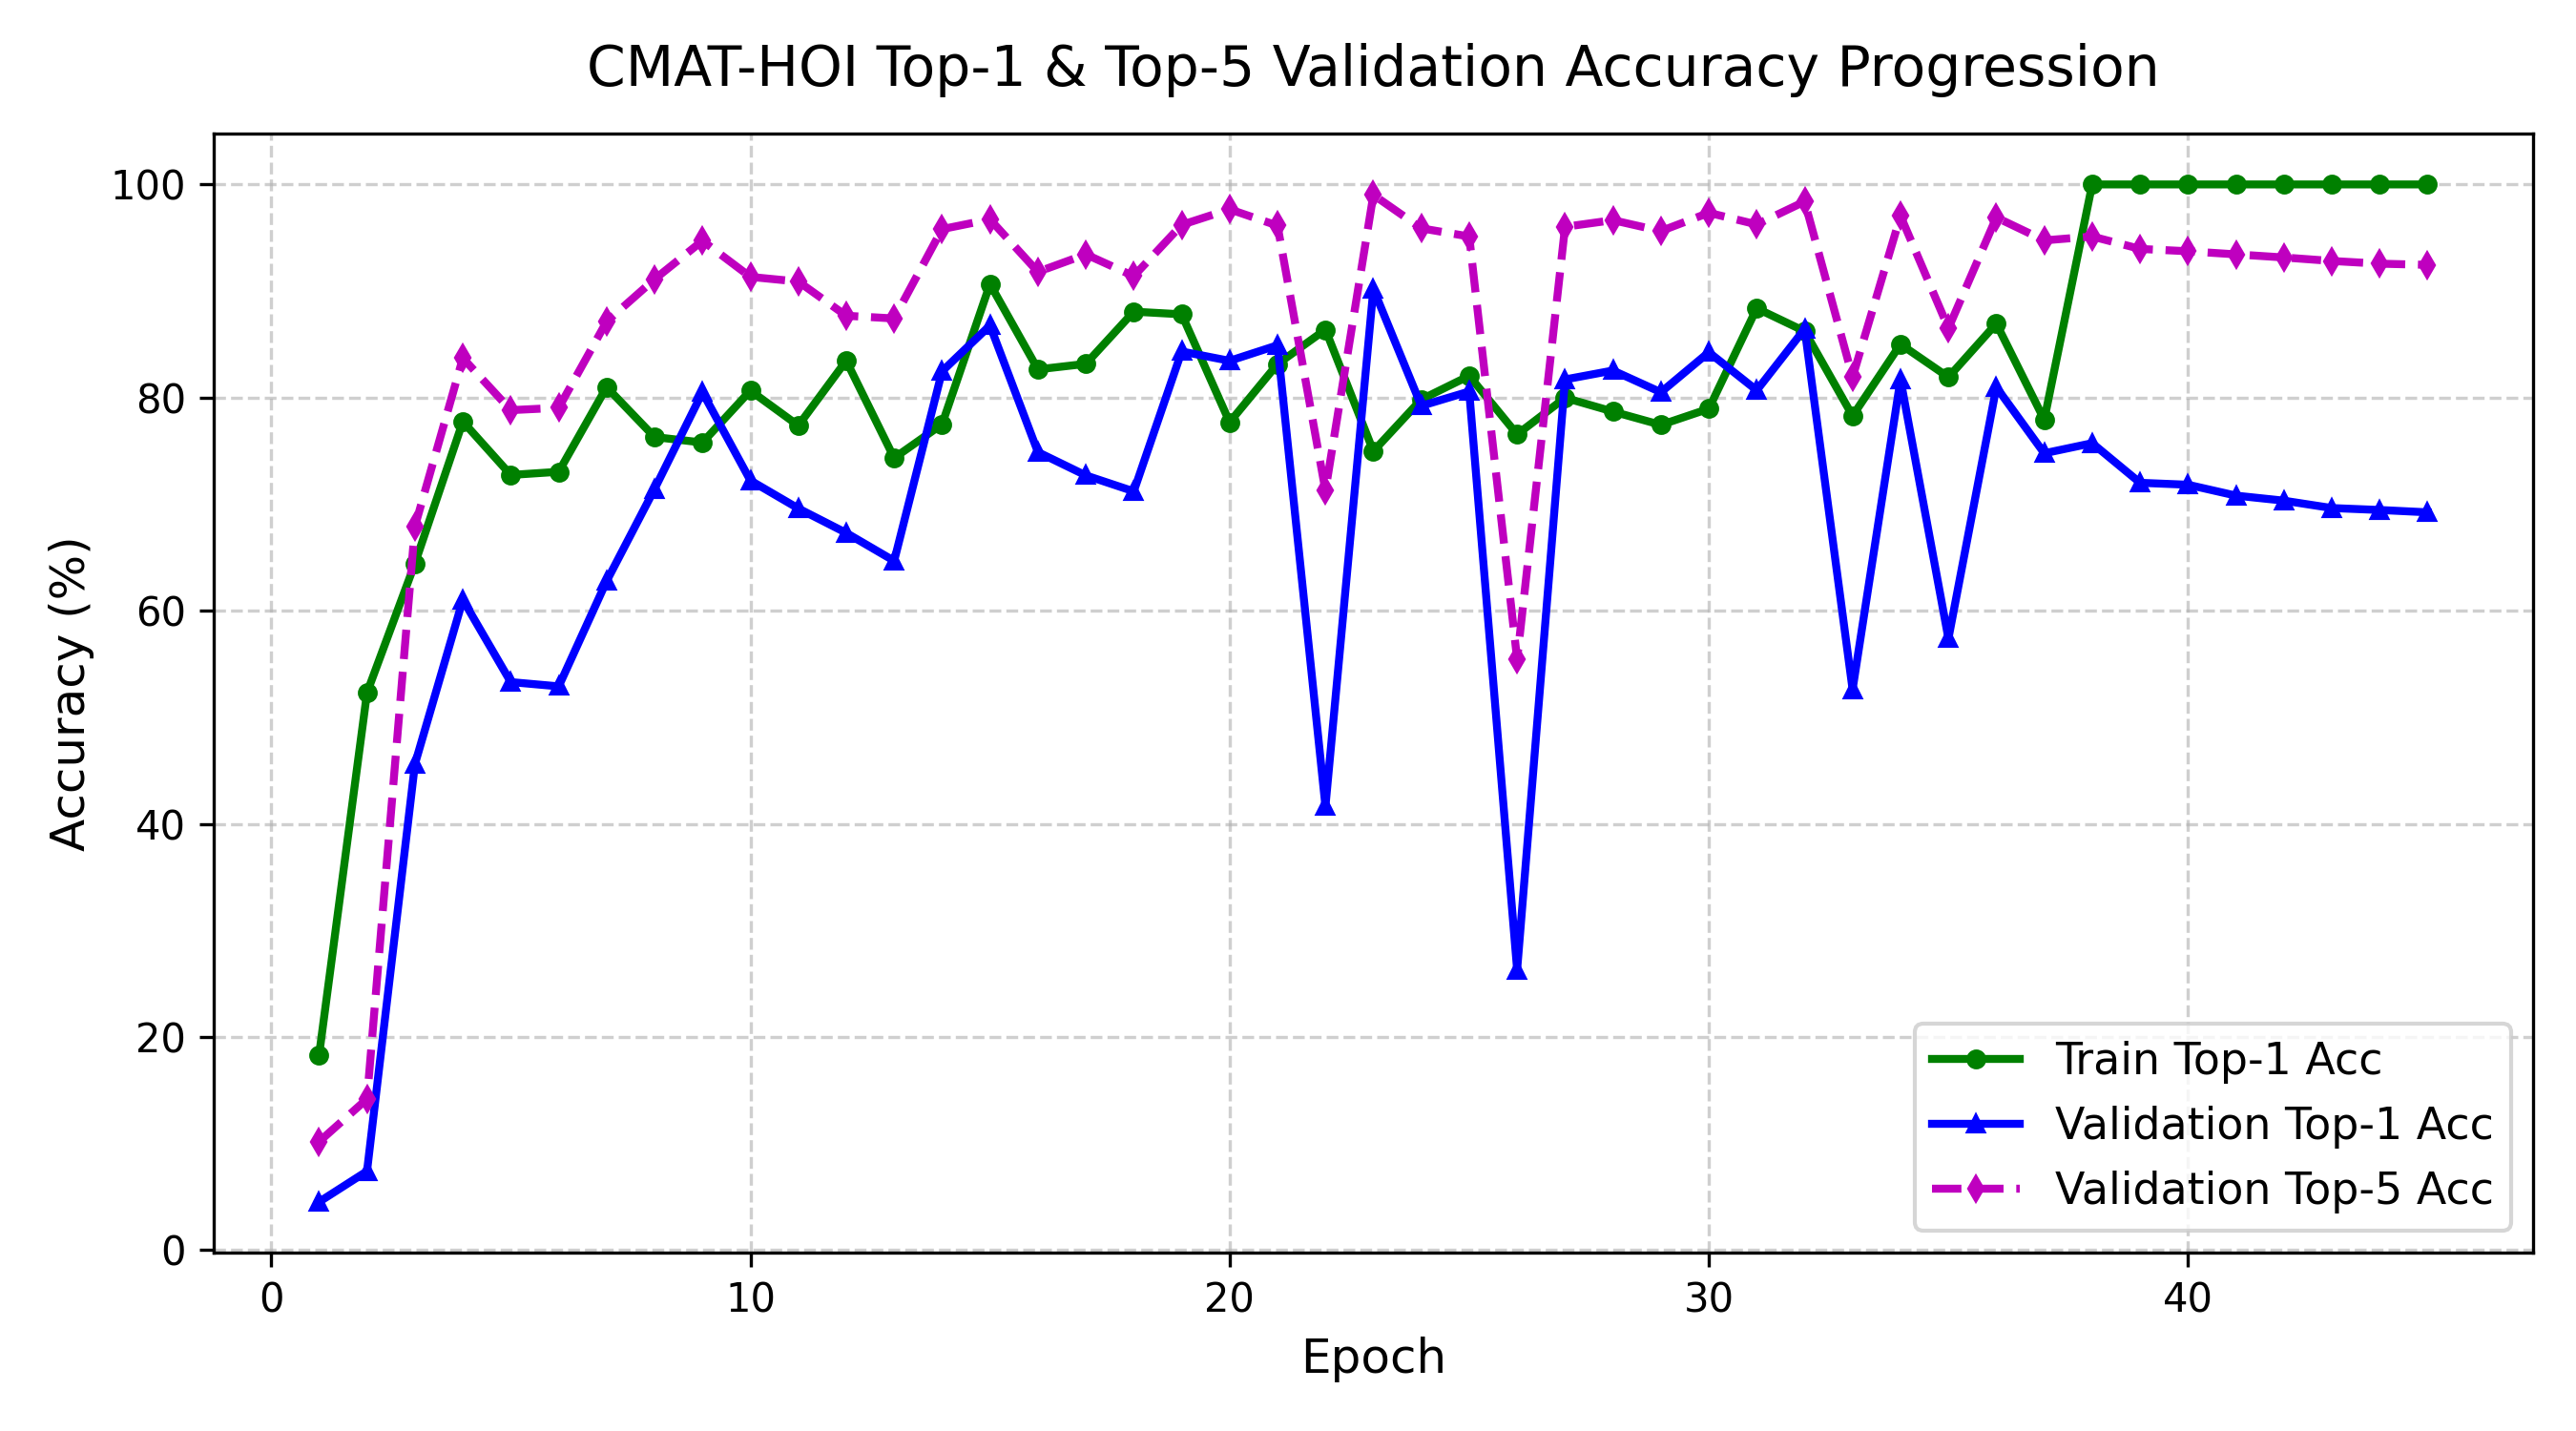
\includegraphics[width=\linewidth]{figures/accuracy_curves.png}
\caption{Training and validation accuracy progression over 45 epochs.}
\label{fig:acc_curves}
\end{figure}

\begin{figure}[t]
\centering
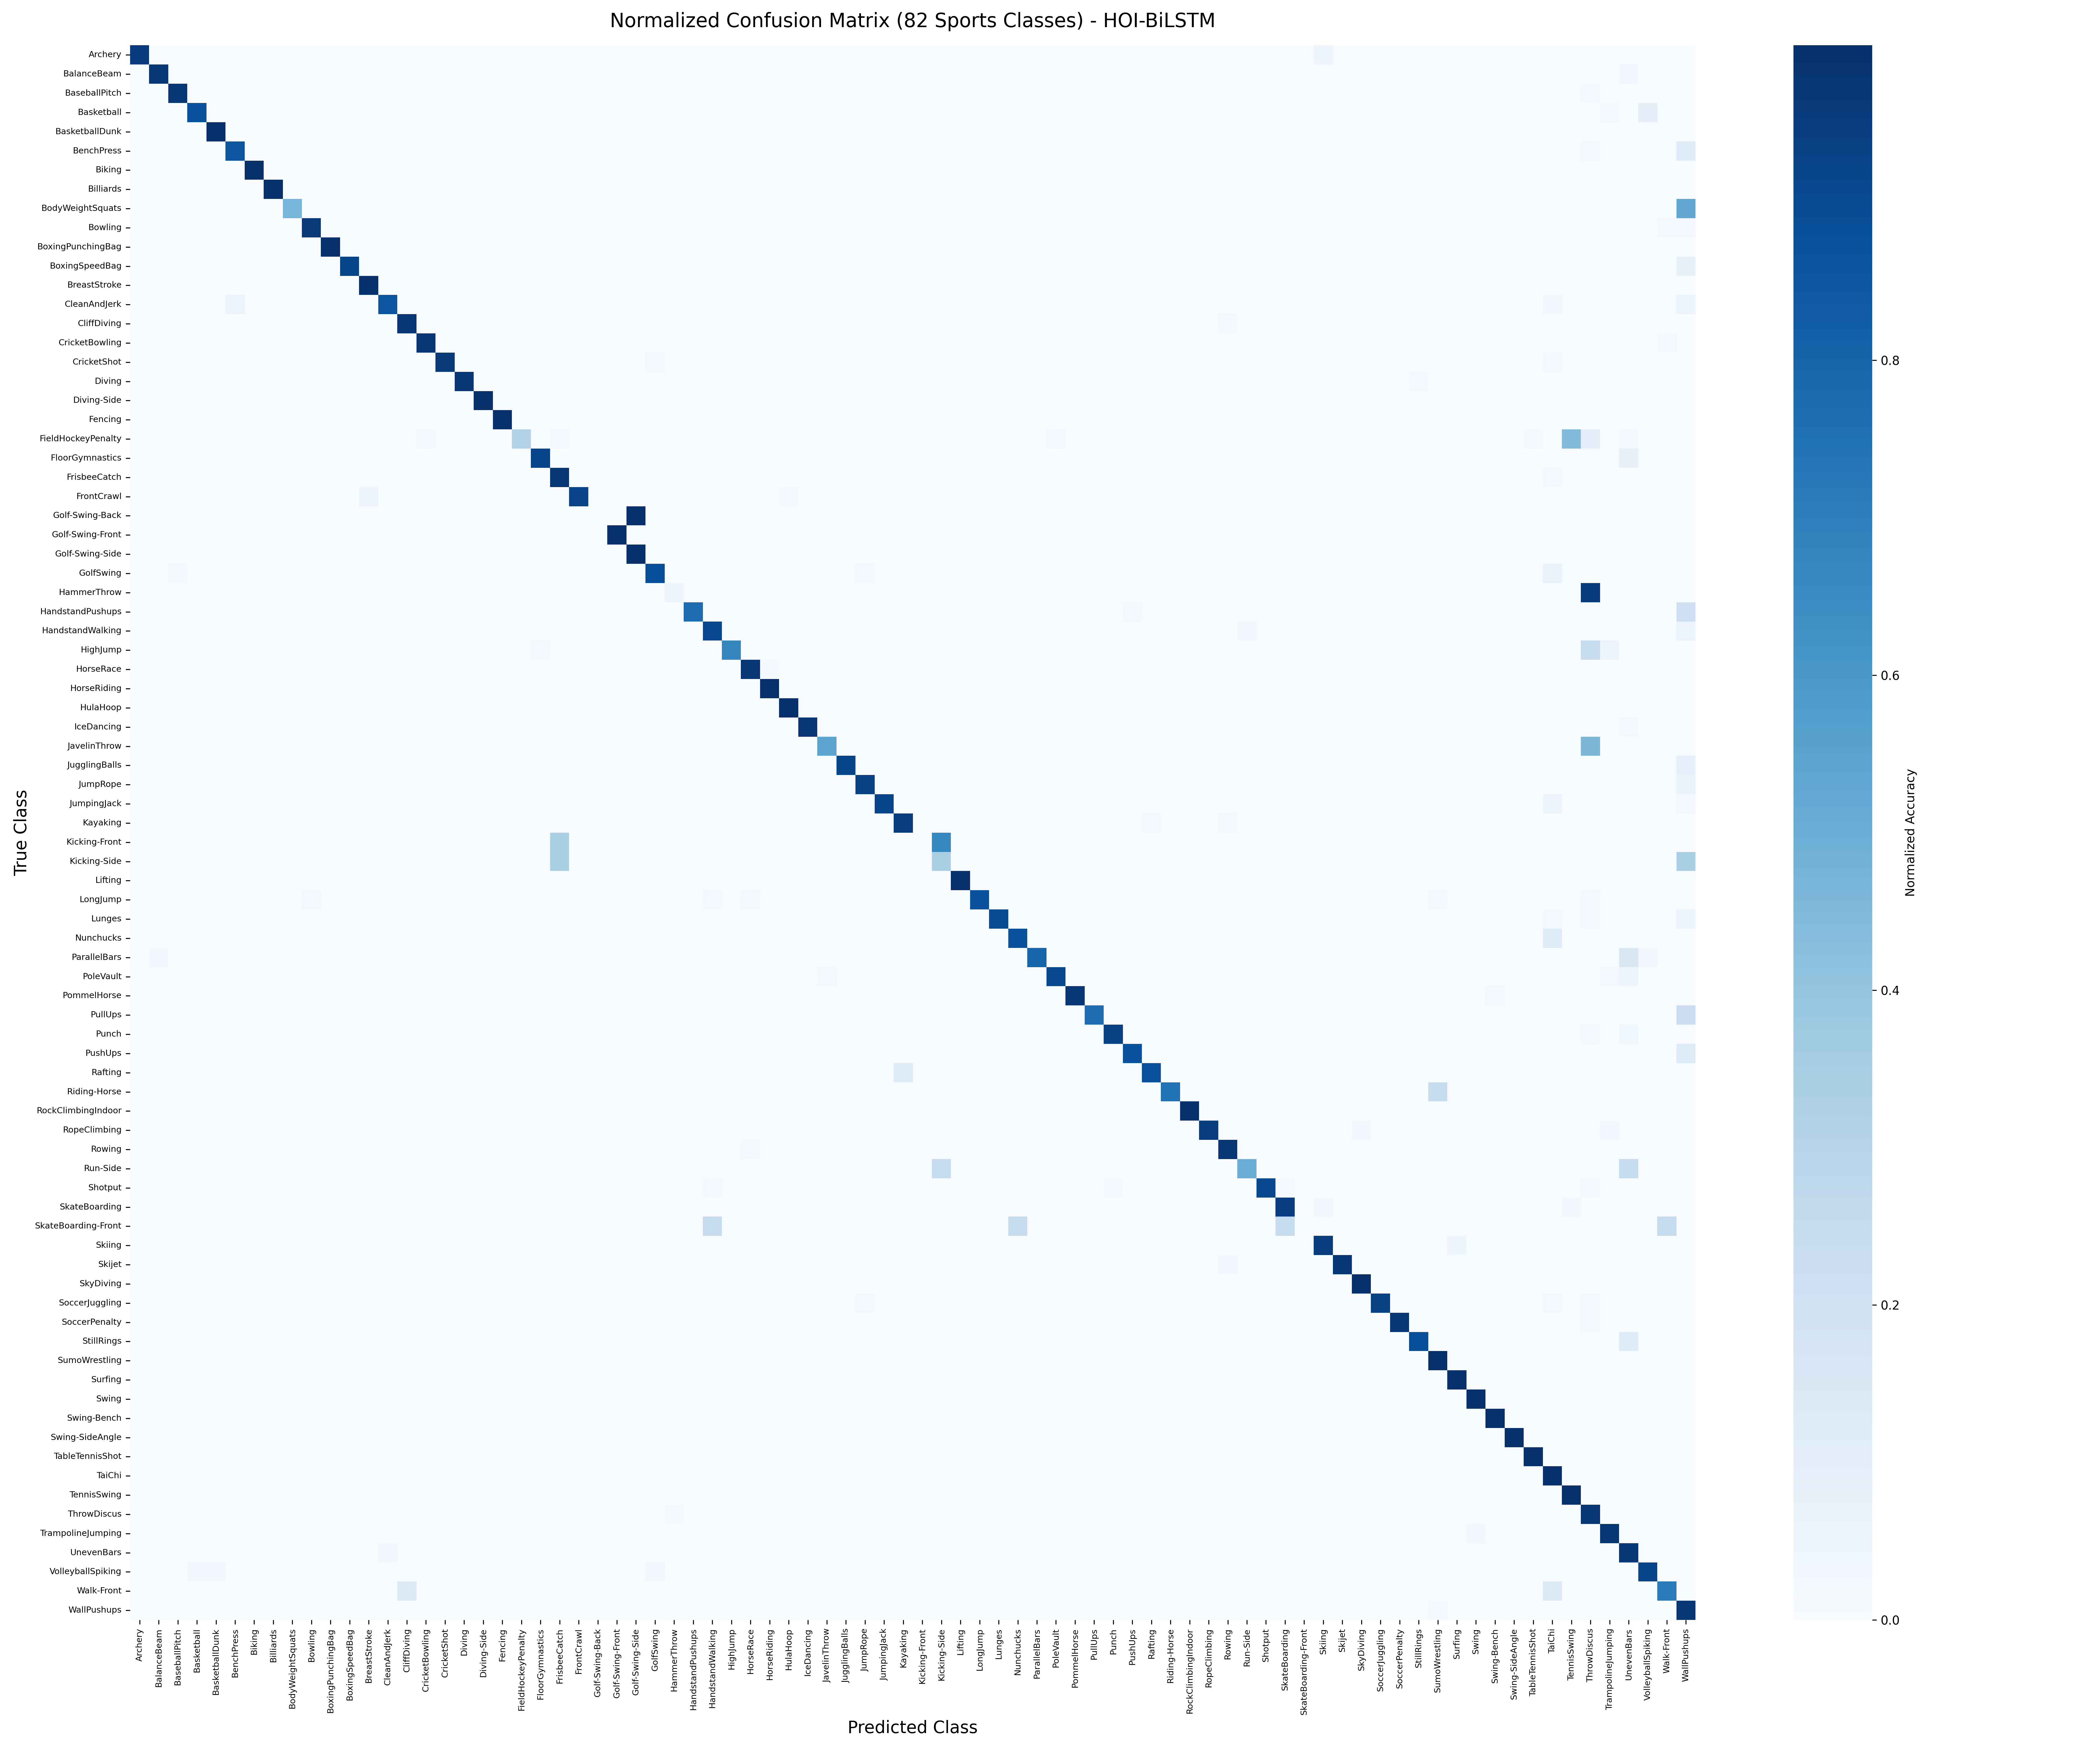
\includegraphics[width=\linewidth]{figures/confusion_matrix_82.png}
\caption{Normalized confusion matrix across all 82 sports categories.}
\label{fig:cm}
\end{figure}

\subsection{Quantitative Performance Comparison}
Table~\ref{tab:comparison} compares CMAT-HOI with the baseline BiLSTM model on the 2,743 test videos.

\begin{table}[h]
\caption{Quantitative Performance on 2,743 Disjoint Test Videos}
\label{tab:comparison}
\centering
\begin{tabular}{lccccc}
\toprule
\textbf{Model} & \textbf{Top-1 (\%)} & \textbf{Top-5 (\%)} & \textbf{Loss} & \textbf{W-F1 (\%)} & \textbf{M-F1 (\%)} \\
\midrule
BiLSTM (M7) & 55.20 & 76.45 & 2.1520 & 54.80 & 48.12 \\
\textbf{CMAT-HOI} & \textbf{90.19} & \textbf{99.02} & \textbf{0.4397} & \textbf{90.19} & \textbf{85.84} \\
\midrule
$\Delta$ & \textbf{+34.99} & \textbf{+22.57} & \textbf{-1.7123} & \textbf{+35.39} & \textbf{+37.72} \\
\bottomrule
\end{tabular}
\end{table}

As shown in Table~\ref{tab:comparison}, CMAT-HOI outperforms the BiLSTM baseline by \textbf{+34.99\% in Top-1 Accuracy} and \textbf{+22.57\% in Top-5 Accuracy}. Peak validation performance was achieved at Epoch 23 with test loss $0.4397$.

\subsection{Ablation Study}
To evaluate the contribution of each modality, we conducted an ablation study (M1 to M7) under identical training protocols (Table~\ref{tab:ablation}).

\begin{table}[h]
\caption{Multimodal Component Ablation Study (M1 to M7)}
\label{tab:ablation}
\centering
\begin{tabular}{cllccc}
\toprule
\textbf{Mode} & \textbf{Configuration} & \textbf{Modalities} & \textbf{Top-1 (\%)} & \textbf{Top-5 (\%)} \\
\midrule
M1 & Visual Only & Visual (ResNet-50) & 68.42 & 84.10 \\
M2 & Pose Only & Keypoints & 52.15 & 71.30 \\
M3 & Object Only & Bounding Boxes & 34.20 & 52.80 \\
M4 & Kinematic HOI & Pose + Object + HOI & 64.75 & 82.50 \\
M5 & Visuo-Kinematic & Visual + Pose & 79.30 & 91.80 \\
M6 & Visuo-Object & Visual + Object & 74.60 & 88.20 \\
\textbf{M7} & \textbf{Full CMAT-HOI} & \textbf{All Streams} & \textbf{90.19} & \textbf{99.02} \\
\bottomrule
\end{tabular}
\end{table}

The ablation results in Table~\ref{tab:ablation} demonstrate that fusing all four streams via Bi-Directional Cross-Attention and GMFU yields a \textbf{+21.77\% gain} over visual-only features (M1) and a \textbf{+38.04\% gain} over pose-only features (M2).

\section{Conclusion}
In this paper, we introduced CMAT-HOI, a Cross-Modal Attention Transformer for fine-grained sports action recognition. CMAT-HOI addresses multimodal representation collapse and scene bias through dimension-aligned modality stems, bi-directional cross-attention between skeletal keypoints and sports apparatus, dynamic gated multimodal fusion, and multi-scale 4-way temporal pooling. Evaluated on an extensive 82-class sports video benchmark of 9,151 clips, CMAT-HOI achieved \textbf{90.19\% Top-1} and \textbf{99.02\% Top-5} accuracy on 2,743 disjoint test videos, outperforming the baseline BiLSTM by \textbf{+34.99\%}.

\bibliographystyle{IEEEtran}
\bibliography{references}

\end{document}
